\documentclass{standalone}

\usepackage{tikz}
\usetikzlibrary{shapes.geometric}
\begin{document}
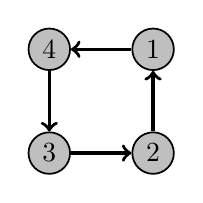
\begin{tikzpicture}
[every node/.style={inner sep=0pt}]
\node (1) [circle, minimum size=15.0pt, fill=lightgray, line width=0.625pt, draw=black] at (75.0pt, -25.0pt) {\textcolor{black}{1}};
\node (2) [circle, minimum size=15.0pt, fill=lightgray, line width=0.625pt, draw=black] at (75.0pt, -62.5pt) {\textcolor{black}{2}};
\node (3) [circle, minimum size=15.0pt, fill=lightgray, line width=0.625pt, draw=black] at (37.5pt, -62.5pt) {\textcolor{black}{3}};
\node (4) [circle, minimum size=15.0pt, fill=lightgray, line width=0.625pt, draw=black] at (37.5pt, -25.0pt) {\textcolor{black}{4}};
\draw [line width=1.25, ->, color=black] (2) to  (1);
\draw [line width=1.25, ->, color=black] (1) to  (4);
\draw [line width=1.25, ->, color=black] (4) to  (3);
\draw [line width=1.25, ->, color=black] (3) to  (2);
\end{tikzpicture}
\end{document}
